\documentclass[fleqn]{article}
\usepackage [utf8] {inputenc}
\usepackage{graphicx}
\RequirePackage{ifthen}            % Test options
\RequirePackage{amsmath,amssymb,bm}% …tendre les fonctions maths
\RequirePackage[frenchb]{babel}    % RËgles typo franÁaises
\begin{document}
\setlength{\fboxsep}{10pt}
\vspace*{-20mm}
\begin{center}
     \centering
	\fbox{
        \begin{minipage}{12cm}
           \centering
            \Large MASTER TACS \\
	    UP1C: Dynamique, vibrations, recalage\\
            \large Projet numérique
        \end{minipage}}
\end{center}


%============================================================================
\vspace{2cm}

\section*{Introduction}

\begin{center}
\begin{minipage}{14cm}
\hspace{1cm} L'objectif de ce "petit" projet numérique est de mettre en application les connaissances découvertes lors du cours intitulé "Dynamique, vibration et recalage". Sur  un léger problème mécanique en dynamique, nous allons donc expliciter quelques différents schémas d'intégration temporelle, une méthode de résolution du problème basée sur les modes propres et une approche du recalage.
 \end{minipage}
\end{center}
%============================================================================
\section{Présentation du problème mécanique et sa résolution par la méthode des éléments finis "classiques"}

%+++++
\subsection{\'Ecriture du problème mécanique}

Cette partie a pour but d'illustrer le problème type sur lequel nous travaillerons ensuite. La figure \ref{PbmBase} illustre la structure support de l'étude: une poutre encastrée à une extrémité ($S_0$) est soumise à un unique chargement $F(t)$ à son autre extrémité ($S_L$).

\begin{figure}[htbp]
	\begin{center}
		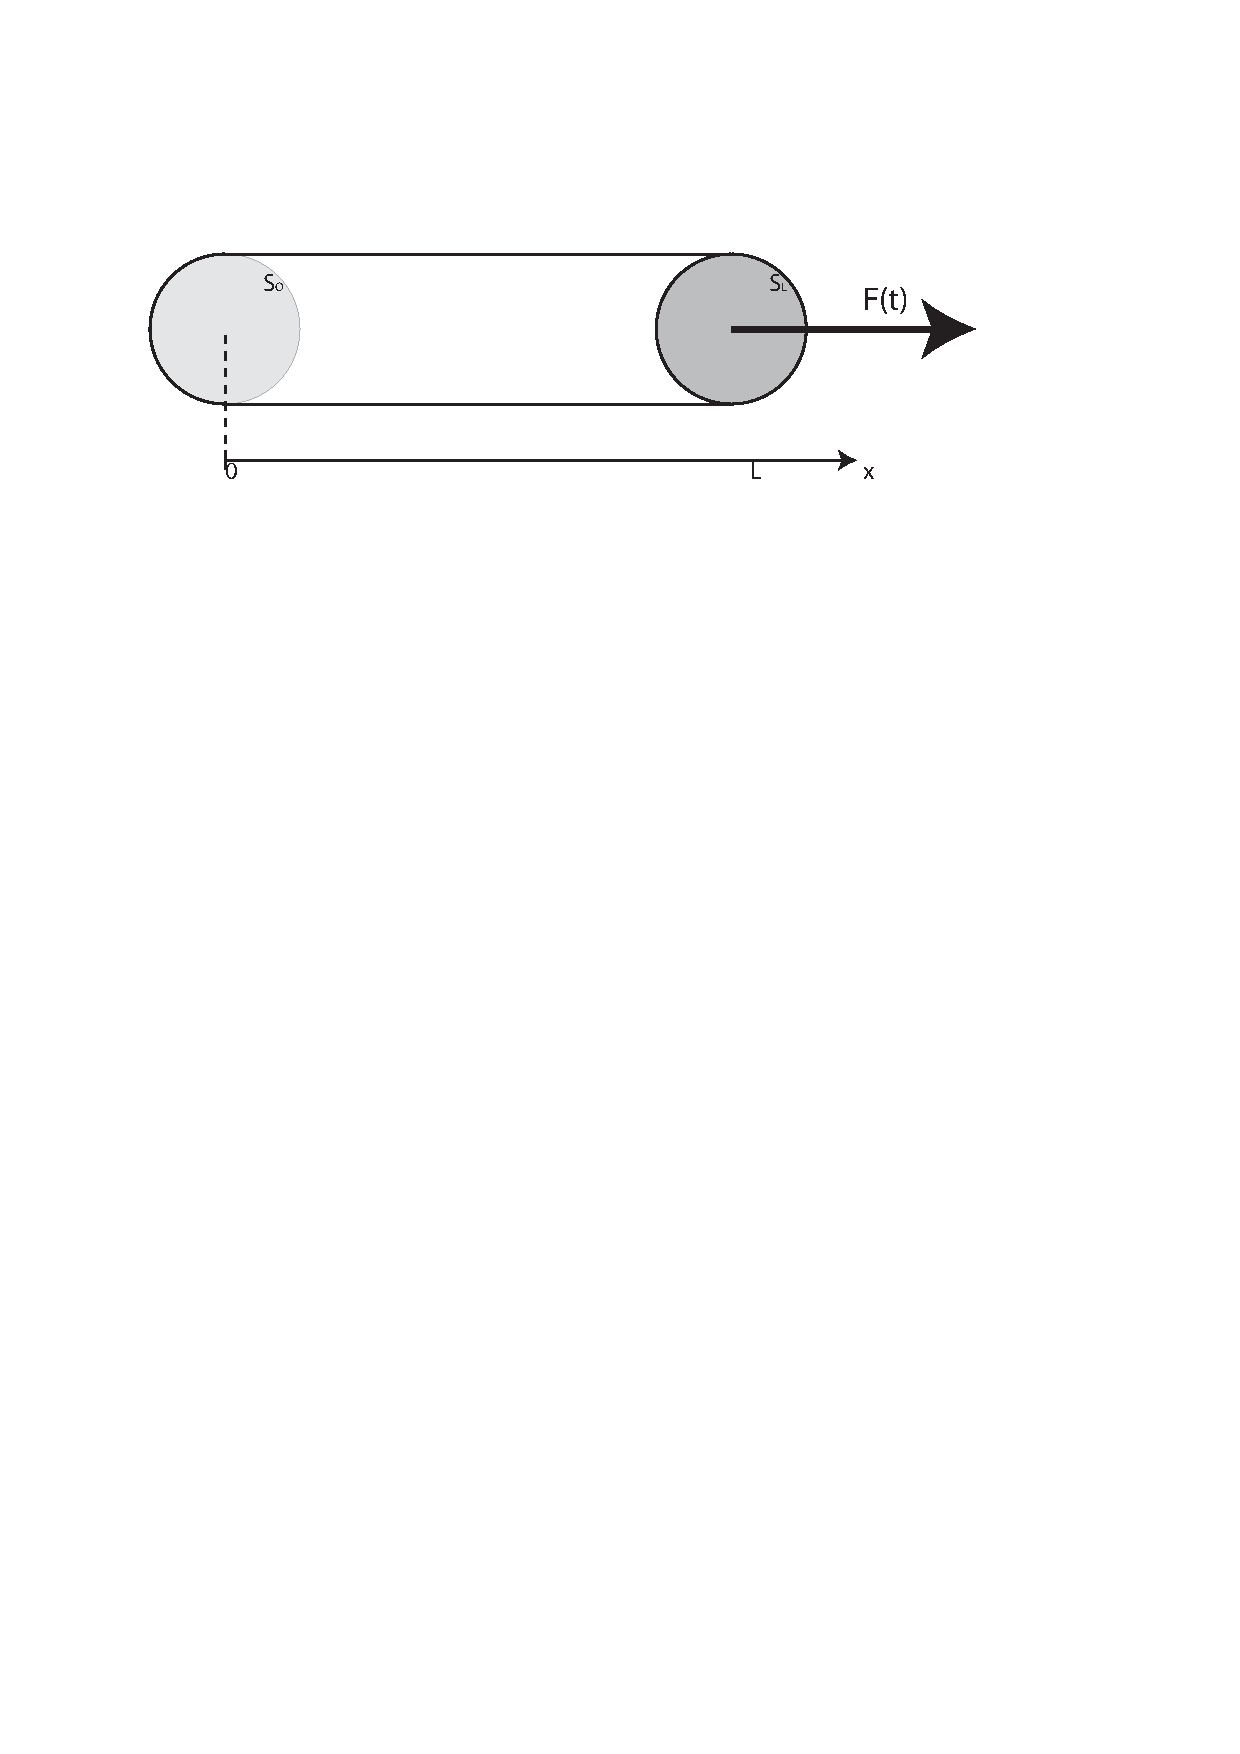
\includegraphics[width=10cm]{figures/poutre_c}
		\caption{Représentation de la structure et de ses interactions avec l'extérieur.}
		\label{PbmBase}
	\end{center}
\end{figure}

Par la suite, on fera les hypothèses de RdM classiques de sortes à ne travailler que sur une poutre de longueur L travaillant en traction-compression et encastrée en son origine $x=0$.

En notant $\rho$ la masse volumique de cette poutre et $\mu$ son coefficient de viscosité, on peut écrire le problème mécanique de la manière suivante:

\begin{it} 
	Trouver le champs de déplacement $U(x,t)$ et la contrainte normale $N(x,t)$ définis sur $\left[0,L\right] \times \left[0,T \right]$ tels que:
\end{it}

\begin{itemize}
	\item Equations de liaison et conditions initiales:
		\begin{equation}
			\begin{array}{l}
				U \in \mathrm{U}^{\left[ 0, T \right]} \\
				\forall t \in \left[ 0,T \right] \quad U(0 ,t)=0 \\
				\forall x \in \left[0,L\right]  \quad U(x,0)=0, \quad \dot{U}(x,0)=0 \mbox{ et } \ddot{U}(x,0)=0
			\end{array}
			\label{eq:CA}
		\end{equation}
	\item Equations d'équilibre:
		\begin{equation}
			\begin{array}{l}
				N \in \mathrm{S}^{\left[ 0, T \right]} \\
				\forall t \in \left[0,T\right] \quad N(L,t)=\frac{F(t)}{S}\\
				\forall (x,t) \in \left[0,L\right] \times \left[ 0,T \right]  \quad \rho S.\ddot{U} = -\mu S.\dot{U} + S.\frac{\partial N}{\partial x} 
			\end{array}
			\label{eq:SA}
		\end{equation}
	\item Relation de comportement:
		\begin{equation}
			\forall (x,t) \in  \left[ 0,L \right] \times \left[ 0,T \right] \quad  N = E \frac{\partial U}{\partial x}
			\label{eq:rdc}
		\end{equation}
\end{itemize}
où les espaces $\mathrm{U}^{\left[ 0, T \right]}$ et $\mathrm{S}^{\left[ 0, T \right]}$ précisent la régularité des champs du déplacement et de contrainte.


\subsubsection{Discrétisation spatiale}

La méthode utilisée pour obtenir une approximation de la solution exacte de ce problème est d'appauvrir les espaces $\mathrm{U}^{\left[ 0, T \right]}$ et $\mathrm{S}^{\left[ 0, T \right]}$. Ainsi l'approche éléments finis classique consiste diviser l'espace d'étude de la manière suivante:

\begin{equation*}
	\left[ 0,L \right]=  \bigcup_{0\leq i<N_e}   \left[ x_i,x_{i+1}\right] \mbox{ avec } x_0=0\mbox{, } x_{N_e}=L  \mbox{ et }  x_i<x_{i+1}\\
\end{equation*}

\begin{figure}[htbp]
	\begin{center}
		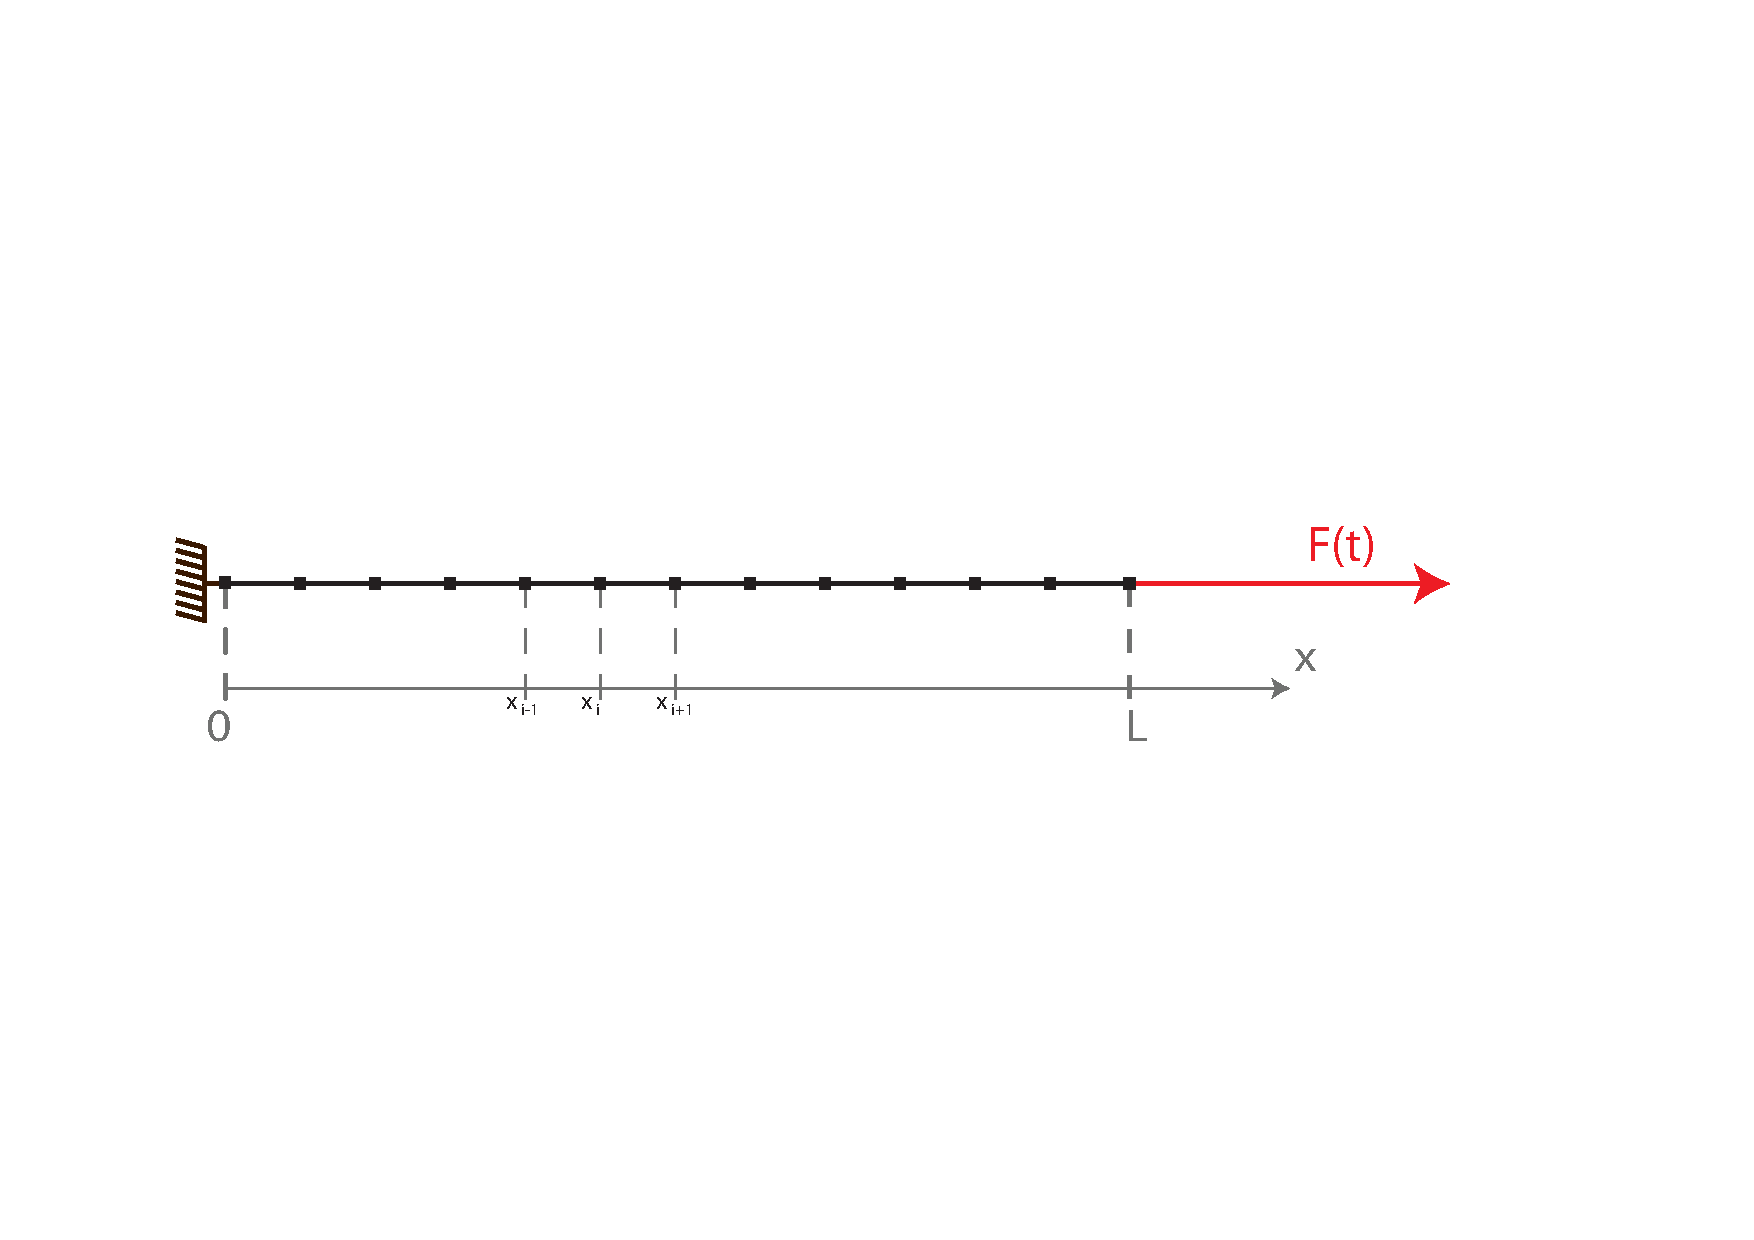
\includegraphics[width=10cm]{figures/poutre_ef}
		\caption{Représentation de la structure discrétisée et de ses interactions avec l'extérieur.}
		\label{PbmBase}
	\end{center}
\end{figure}

On réduit alors l'espace de recherche du déplacement à:
\begin{equation*}
	\mathrm{U}^{\left[ 0, T \right]}_e=\{  U \mbox{ tel que } U \mbox{ continu sur }\left[ 0, L \right] \mbox{ et linéaire sur } \left[ x_i,x_{i+1}\right]\forall i  \mbox{ tq } 0 \leq i < N_e \}
\end{equation*}
On en déduit $\mathrm{S}^{\left[ 0, T \right]}_h=\epsilon(\mathrm{U}^{\left[ 0, T \right]}_h)$.
La discrétisation spatiale du problème permet d'écrite alors le problème mécanique sous sa forme classique:

\begin{it} 
	Trouver le vecteur des déplacements nodaux $\underline{U}(t)$ tels que:
\end{it}
\begin{itemize}
	\item Equation de liaison et conditions initiales:
		\begin{equation*}
			\begin{array}{l}
				\forall t \in \left[0,T\right] \quad U_0(t)=0\\
				\forall x \in \left[0,L\right] \quad \underline{U}=0, \underline{\dot{U}}=0 \mbox{ et }\underline{\ddot{U}}=0
			\end{array}
		\end{equation*}
	\item Equation d'équilibre (écriture sous forme matricielle):
		\begin{equation*}
			\underline{\underline{M}}.\underline{\ddot{U}}(t) + \underline{\underline{C}}.\underline{\dot{U}}(t) + \underline{\underline{K}}.\underline{U}(t) = \underline{F}(t)
		\end{equation*}
\end{itemize}
	Où $\underline{\underline{M}}$, $\underline{\underline{K}}$, $\underline{\underline{C}}$ et $\underline{F}$ sont respectivement les matrices de masse, de rigidité, d'amortissement et l'effort généralisé du problème discrétisé. 
	Par la suite,  on travaillera avec la définition de la matrice de rigidité suivante: $\underline{\underline{C}}=\alpha.\underline{\underline{M}} +\beta.\underline{\underline{K}}$ avec $\alpha$ et $\beta$ deux paramètres.


Ensuite on en déduit la contrainte normale dans chacun des éléments à l'aide de la relation de comportement:
		\begin{equation*}
			\forall t \in \left[ 0,T \right] \quad  N_i(t) = E \frac{U_{i}(t)-U_{i-1}(t)}{x_{i+1}-x_i} \mbox{ } \forall i \mbox{ tq } 0\leq i\leq N_e
		\end{equation*}

\subsubsection{Discrétisation temporelle}

La méthode des éléments finis classique appauvrie aussi l'espace de fonction dans lequel on va chercher le déplacement au sens temporel; on peut définir alors le nouvelle espace de recherche:

\begin{equation*}
	\mathrm{U}^{\left[ 0, T \right]}_{ef}=\{  U \mbox{ tel que } U \mbox{ continu sur }\left[ 0, L \right]\times\left[0,T\right] \mbox{ et linéaire sur } \left[ x_i,x_{i+1}\right]\times \left[ t_n,t_{n+1}\right]\}
\end{equation*}
Avec
\begin{equation*}
	\left[ 0,T \right]=  \bigcup_{0\leq n<N_t}   \left[t_n,t_{n+1}\right] \mbox{ avec } t_0=0 \mbox{, } t_{N_t}=T  \mbox{ et } t_n<t_{n+1}
\end{equation*}
		
La méthode choisie pour résoudre ce problème sur l'intervalle de temps $\left[0,T\right]$ est une méthode dite incrémentale: on suppose connue les valeurs de toutes les grandeurs définissant l'évolution du problème pour $t \in \left[0,t_n\right]$, et on cherche leur valeur au pas de temps $t_{n+1}$. Leur évolution est définie par l'espace de recherche: le champs de déplacement a une évolution linéaire entre chaque pas de temps. Le problème devient donc:

\begin{it} 
	Trouver le vecteur des déplacements nodaux $\underline{U}(t_{n+1})$ tels que:
\end{it}
\begin{itemize}
	\item Equation de laison:
		\begin{equation*}
			\begin{array}{l}
				\forall t \in \left[0,T\right] \quad U_0(t_{n+1})=0\\
			\end{array}
		\end{equation*}
	\item Equation d'équilibre (écriture sous forme matricielle):
		\begin{equation*}
			\underline{\underline{M}}.\underline{\ddot{U}}(t_{n+1}) + \underline{\underline{C}}.\underline{\dot{U}}(t_n{+1}) + \underline{\underline{K}}.\underline{U}(t_{n+1}) = \underline{F}(t_{n+1})
		\end{equation*}
\end{itemize}

Puis le calcul de la contrainte:
		\begin{equation*}
			\forall t \in \left[ 0,T \right] \quad  N_i(t) = E \frac{U_{i}(t)-U_{i-1}(t)}{x_{i+1}-x_i} \mbox{ } \forall i \mbox{ tq } 0\leq i\leq N_e
		\end{equation*}

Il faut maintenant choisir une méthode d'intégration de sorte à exprimer les dérivées successives de $\underline{U}(t_{n+1})$ en fonction de $(\underline{U}(t_k))$, $k\leq n+1$. On choisit tout d'abord la méthode d'Euler arrière:
\begin{equation*}
	\underline{\dot{U}}(t_{n+1}) = \frac{\underline{U}(t_{n+1})-\underline{U}(t_n)}{t_{n+1}-t_n} \mbox{ et } \underline{\ddot{U}}(t_{n+1}) = \frac{\underline{\dot{U}}(t_{n+1})-\underline{\dot{U}}(t_n)}{t_{n+1}-t_n}
\end{equation*}

En supposant l'écarts entre tous les pas de temps égaux à $dt$, le problème au pas de temps $t_{n+1}$ s'écrit donc:

\begin{it} 
	Trouver le vecteur des déplacements nodaux $\underline{U}(t_{n+1})$ tels que:
\end{it}
\begin{itemize}
	\item Equation de laison:
		\begin{equation*}
			\begin{array}{l}
				\forall t \in \left[0,T\right] \quad U_0(t_{n+1})=0\\
			\end{array}
		\end{equation*}
	\item Equation d'équilibre (écriture sous forme matricielle):
		\begin{equation*}
			\underline{U}(t_{n+1}) = f(\underline{U}(t_n))+g(\underline{U}(t_{n-1})) +\underline{F}(t_{n+1})
		\end{equation*}
\end{itemize}

Système linéaire classique à résoudre qui nous permet de déterminer le déplacement de chacun des noeuds du problème au temps $t_{n+1}$, on pourra alors en déduire la contrainte dans chacun des éléments à ce même instant.

Cette méthode de résolution codée en Matlab est disponible sur \\ "/utmp/tibouren/kovalevsky/SourcesTACS/".

\section{Travail demandé}

\subsection{Résolution sur la base des modes propres}

On peut "facilement" déterminer les premiers modes propres d'une structure; et on peut alors résoudre le problème EF non plus sur la base des fonctions de forme classique mais sur une base des premiers modes propres. 
A l'aide du problème éléments finis déterminer les premiers modes propres de la poutre. 
Résoudre le problème dans une base construite avec les premiers modes propres, en concidérant un effort en bout de poutre de type échelon.

 Étudier le nombre de mode nécessaire à une bonne approximation de la solution et expliquer pourquoi trop de modes polluent la solution. 

\subsection{Etude de différents schéma d'intégration}

Calculer la solution du problème de dynamique en introduisant deux schémas d'intégrations un implicite, et un autre explicite pour les différents chargements $F(t)$ en bout de poutre.

\begin{itemize}
	\item chargement en créneaux;
	\item chargement du type échelon;
	\item chargement en rampe;
	\item chargement harmonique (sinus).
\end{itemize}

Conclure.




\end{document}
